\begin{song}{title=\centering Zatanči \\\normalsize Jaromír Nohavica  \vspace*{-0.3cm}}  %% sem se napíše jméno songu a autor
\moveright \stred \vbox{      %Varianta č. 1  ---> Jeden sloupec zarovnaný na střed	

\sloka
^{Emi G}Zatanči, má milá, ^{D{\color{white}\_\_}}zatanči ^{Emi}pro mé oči,

^{{\color{white}\_\_}G}zatanči a vetkni nůž ^{D}do mých ^{Emi}zad,

ať tvůj ^{G}šat, má milá, ať ^{D}tvůj šat ^{Emi}na zemi skončí,

ať tvůj ^{G}šat, má milá, ^{D}rázem je ^{Emi}sňat.

\refren
^{Emi G}Zatanči, jako se ^{D{\color{white}\_}}okolo ^{Emi\,\,}ohně tančí,

^{{\color{white}\_\_}G}zatanči jako ^{D{\color{white}\_\_}}navodě ^{Emi}loď,

^{{\color{white}\_\_}G}zatanči jako to ^{D}slunce ^{Emi}mezi pomeranči,

^{{\color{white}\_\_}G}zatanči, a ^{D}pak ke mně ^{Emi}pojď.

\phantom{.}

[Mezihra]

\sloka
Polož dlaň, má milá, polož dlaň na má prsa,

polož dlaň nestoudně na moji hruď,

obejmi, má milá, obejmi moje bedra,

obejmi je pevně a mojí buď.

\refren

\phantom{.}

[Mezihra]

\sloka
Nový den než začne, má milá, nežli začne,

nový den než začne, nasyť můj hlad,

zatanči, má milá, pro moje oči lačné,

zatanči a já budu ti hrát.

\refren

\refren
}
\setcounter{Slokočet}{0}
\end{song}

\begin{figure}[h]
\centering
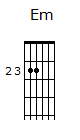
\includegraphics[scale=1.5]{../Akordy/em.png} 
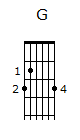
\includegraphics[scale=1.5]{../Akordy/g.png}
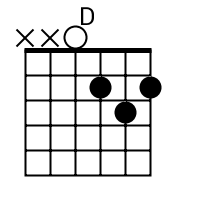
\includegraphics[scale=1.5]{../Akordy/d.png}
\end{figure}